\documentclass[border=1pt]{standalone}
\usepackage{tikz}
\usetikzlibrary{arrows.meta,calc}

\begin{document}
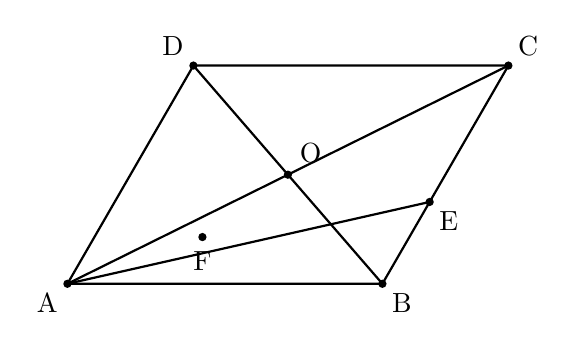
\begin{tikzpicture}[x=4mm, y=4mm]

    % 平行四辺形ABCD
    % A(0,0), B(10,0), C(14,6.928), D(4,6.928)
    % AB=10, BC=8, ∠ABC=60°
    
    \coordinate (A) at (0,0);
    \coordinate (B) at (10,0);
    \coordinate (C) at (14,6.928);
    \coordinate (D) at (4,6.928);
    
    % 辺BC上の点E: BE=3
    % E = B + (3/8)*(C-B)
    \coordinate (E) at (11.5,2.598);
    
    % 対角線の交点O
    \coordinate (O) at (7,3.464);
    
    % 線分AEと線分BDの交点F
    \coordinate (F) at (4.286,1.484);
    
    % 平行四辺形の描画
    \draw[thick] (A) -- (B) -- (C) -- (D) -- cycle;
    
    % 対角線
    \draw[thick] (A) -- (C);
    \draw[thick] (B) -- (D);
    
    % 線分AE
    \draw[thick] (A) -- (E);
    
    % 点のマーク
    \fill (A) circle (1.5pt) node[below left] {$\mathrm{A}$};
    \fill (B) circle (1.5pt) node[below right] {$\mathrm{B}$};
    \fill (C) circle (1.5pt) node[above right] {$\mathrm{C}$};
    \fill (D) circle (1.5pt) node[above left] {$\mathrm{D}$};
    \fill (E) circle (1.5pt) node[below right] {$\mathrm{E}$};
    \fill (O) circle (1.5pt) node[above right, outer sep=1pt] {$\mathrm{O}$};
    \fill (F) circle (1.5pt) node[below, outer sep=2pt] {$\mathrm{F}$};

\end{tikzpicture}
\end{document}
